\section{Stabla}

% 1.zadatak
\begin{Exercise}[label=4_14]
Napisati biblioteku za rad sa binarnim pretraživačkim stablima.

\begin{enumerate}
\item Definisati strukturu \kckod{Cvor} kojom se opisuje čvor stabla, a koja sadrži ceo broj \kckod{broj} i pokazivače \kckod{levo} i \kckod{desno} redom na levo i desno podstablo.

\item Napisati funkciju \kckod{Cvor *napravi\_cvor(int broj)} koja alocira memoriju za novi čvor stabla i vrši njegovu inicijalizaciju zadatim celim brojem \argf{broj}.

\item Napisati funkciju \kckod{int dodaj\_u\_stablo(Cvor ** adresa\_korena, int broj)} koja u stablo na koje pokazuje argument \argf{adresa\_korena} dodaje ceo broj \argf{broj}. Povratna vrednost funkcije je $0$ ako je dodavanje uspešno, odnosno $1$ ukoliko je došlo do greške.  

\item Napisati funkciju \kckod{Cvor *pretrazi\_stablo(Cvor * koren, int broj)} koja proverava da li se ceo broj \argf{broj} nalazi u stablu sa korenom \argf{koren}. Funkcija vraća pokazivač na čvor stabla koji sadrži traženu vrednost ili $NULL$ ukoliko takav čvor ne postoji.

\item Napisati funkciju \kckod{Cvor *pronadji\_najmanji(Cvor * koren)} koja pronalazi čvor koji sadrži najmanju vrednost u stablu sa korenom \argf{koren}. 

\item Napisati funkciju \kckod{Cvor *pronadji\_najveci(Cvor * koren)} koja pronalazi čvor koji sadrži najveću vrednost u stablu sa korenom \argf{koren}.

\item Napisati funkciju \kckod{void obrisi\_element(Cvor ** adresa\_korena, int broj)} koja briše čvor koji sadrži vrednost \argf{broj} iz stabla na koje pokazuje argument \argf{adresa\_korena}.

\item Napisati funkciju \kckod{void ispisi\_stablo\_infiksno(Cvor * koren)} koja infiksno ispisuje sadržaj stabla sa korenom \argf{koren}. Infiksni ispis podrazumeva ispis levog podstabla, korena, a zatim i desnog podstabla.

\item Napisati funkciju \kckod{void ispisi\_stablo\_prefiksno(Cvor * koren)} koja prefiksno ispisuje sadržaj stabla sa korenom \argf{koren}. Prefiksni ispis podrazumeva ispis korena, levog podstabla, a zatim i desnog podstabla.

\item Napisati funkciju \kckod{void ispisi\_stablo\_postfiksno(Cvor * koren)} koja postfiksno ispisuje sadržaj stabla sa korenom \argf{koren}. Postfiksni ispis podrazumeva ispis levog podstabla, desnog podstabla, a zatim i korena.

\item Napisati funkciju \kckod{void oslobodi\_stablo(Cvor ** adresa\_korena)} koja oslobađa memoriju zauzetu stablom na koje pokazuje argument \argf{adresa\_korena}.
\end{enumerate}

Korišćenjem kreirane biblioteke, napisati program koji sa standardnog ulaza učitava cele brojeve sve do kraja ulaza, dodaje ih u binarno pretraživačko stablo i ispisuje stablo u svakoj od navedenih notacija. Zatim omogućiti unos još dva cela broja i demonstrirati rad funkcije za pretragu nad prvim unetim brojem i rad funkcije za brisanje elemenata nad drugim unetim brojem. 

\begin{miditest}
\begin{upotreba}{1}
#\naslovInt#
#\izlaz{Unesite brojeve (CRL+D za kraj unosa):}#
#\ulaz{7 2 1 9 32 18}#
#\izlaz{Infiksni ispis: 1 2 7 9 18 32}#
#\izlaz{Prefiksni ispis: 7 2 1 9 32 18}#
#\izlaz{Postfiksni ispis: 1 2 18 32 9 7}#
#\izlaz{Trazi se broj:}\ulaz{11}#
#\izlaz{Broj se ne nalazi u stablu!}#
#\izlaz{Brise se broj:}\ulaz{7}#
#\izlaz{Rezultujuce stablo: 1 2 9 18 32}#
\end{upotreba}
\end{miditest}
\begin{miditest}
\begin{upotreba}{2}
#\naslovInt#
#\izlaz{Unesite brojeve (CRL+D za kraj unosa):}#
#\ulaz{8 -2 6 13 24 -3}#
#\izlaz{Infiksni ispis:  -3 -2 6 8 13 24}#
#\izlaz{Prefiksni ispis: 8 -2 -3 6 13 24}#
#\izlaz{Postfiksni ispis: -3 6 -2 24 13 8}#
#\izlaz{Trazi se broj:}\ulaz{6}#
#\izlaz{Broj se nalazi u stablu!}#
#\izlaz{Brise se broj:}\ulaz{14}#
#\izlaz{Rezultujuce stablo: -3 -2 6 8 13 24}#
\end{upotreba}
\end{miditest}

\linkresenje{4_14}
\end{Exercise}

\begin{Answer}[ref=4_14]
\includecodeLib{resenja/biblioteke/stabla/stabla.h}{stabla.h}
\includecodeLib{resenja/biblioteke/stabla/stabla.c}{stabla.c}
\includecodeLib{resenja/4_DinamickeStrukture/4_14.c}{main.c}
\end{Answer}

%2.zadatak
\begin{Exercise}[label=4_15]
Napisati program koji izračunava i na standardni izlaz ispisuje broj pojavljivanja svake reči datoteke čije se ime zadaje kao argument komandne linije. Program realizovati korišćenjem binarnog pretraživačkog stabla uređenog leksikografski po rečima ne uzimajući u obzir razliku između malih i velikih slova. Ukoliko prilikom pokretanja programa korisnik ne navede ime ulazne datoteke ispisati na standardni izlaz za grešku poruku $Nedostaje\ ime\ ulazne\ datoteke!$. Može se pretpostaviti da dužina reči neće biti veća od $50$ karaktera.

\begin{miditest}
\begin{test}{1}
#\poziv{./a.out test.txt}#
  
#\naslovDat{test.txt}#
#\datoteka{Sunce utorak raCunar SUNCE programiranje}#
#\datoteka{jabuka PROGramiranje sunCE JABUka}#

#\naslovIzlaz#
#\izlaz{jabuka: 2}#
#\izlaz{programiranje: 2}#
#\izlaz{racunar: 1}#
#\izlaz{sunce: 3}#
#\izlaz{utorak: 1}#
#\izlaz{}#
#\izlaz{Najcesca rec: sunce (pojavljuje se 3 puta)}#
\end{test}
\end{miditest}
\begin{miditest}
\begin{test}{2}
#\poziv{./a.out suma.txt}#

#\naslovDat{suma.txt}#
#\datoteka{lipa zova hrast ZOVA breza LIPA}#

#\naslovIzlaz#
#\izlaz{breza: 1}#
#\izlaz{hrast: 1}#
#\izlaz{lipa: 2}#
#\izlaz{zova: 2}#
#\izlaz{}#
#\izlaz{Najcesca rec: lipa}#
#\izlaz{(pojavljuje se 2 puta)}#
\end{test}
\end{miditest}

\begin{miditest}
\begin{test}{3}
#\poziv{./a.out ulaz.txt}#

#\naslovDat{Datoteka ulaz.txt ne postoji}#

#\naslovIzlazZaGresku#
#\izlaz{Greska: Neuspesno otvaranje datoteke ulaz.txt.}#
\end{test}
\end{miditest}
\begin{miditest}
\begin{test}{4}
#\poziv{./a.out}#
  
#\naslovIzlazZaGresku#
#\izlaz{Greska: Nedostaje ime ulazne datoteke!}#
\end{test}
\end{miditest}
\linkresenje{4_15}
\end{Exercise}

\begin{Answer}[ref=4_15]
\includecode{resenja/4_DinamickeStrukture/4_15.c}
\end{Answer}

%3.zadatak

%4.zadatak
\begin{Exercise}[label=4_16]
U svakoj liniji datoteke čije se ime zadaje sa standardnog ulaza nalazi se ime osobe, prezime osobe i njen broj telefona međusobno razdvojeni blanko znakom, na primer $Milos\ Peric\ 064/123-4567$.  Napisati program koji korišćenjem binarnog pretraživačkog stabla implementira mapu koja sadrži navedene informacije i koja će omogućiti pretragu brojeva telefona za zadata imena i prezimena. Imena i prezimena se unose sve do unosa reči $KRAJ$, a za svaki od unetih podataka ispisuje se ili broj telefona ili obaveštenje da traženi broj nije u imeniku. Može se pretpostaviti da imena, prezimena i brojevi telefona neće biti duži od $30$ karaktera, kao i da imenik ne sadrži podatke o osobama sa istim imenom i prezimenom.

\begin{miditest}
\begin{upotreba}{1}
#\naslovDat{imenik.txt}#  
#\datoteka{Milos Peric 011/3240-987}#
#\datoteka{Marko Maric 064/1234-987}#
#\datoteka{Mirko Maric 011/589-333}#
#\datoteka{Sanja Savkovic 063/321-098}#
#\datoteka{Zika Zikic 021/759-858}#
          
#\naslovInt#
#\izlaz{Unesite ime datoteke:}\ulaz{imenik.txt}#
#\izlaz{Unesite ime i prezime:}\ulaz{Milos Peric}#	
#\izlaz{Broj je: 011/3240-987}#
#\izlaz{Unesite ime i prezime:}\ulaz{Marko Markovic}#
#\izlaz{Broj nije u imeniku!}#
#\izlaz{Unesite ime i prezime:}\ulaz{KRAJ}#
\end{upotreba}
\end{miditest}
\begin{miditest}
\begin{upotreba}{2}
#\naslovDat{Datoteka imenik1.txt ne postoji}#
  
#\naslovInt#
#\izlaz{Unesite ime datoteke:}\ulaz{imenik1.txt}#
#\naslovIzlazZaGresku#
#\izlaz{Greska: Neuspesno otvaranje datoteke}#
#\izlaz{imenik1.txt.}#
\end{upotreba}
\end{miditest}
\linkresenje{4_16}
\end{Exercise}

\begin{Answer}[ref=4_16]
\includecode{resenja/4_DinamickeStrukture/4_16.c}
\end{Answer}

%5.zadatak
\begin{Exercise}[label=4_17]
U datoteci \kckod{prijemni.txt} nalaze se podaci o prijemnom ispitu učenika jedne osnovne škole tako što je u svakom redu navedeno ime i prezime učenika (niska od najviše $50$ karaktera), broj poena na osnovu uspeha (realan broj), broj poena na prijemnom ispitu iz matematike (realan broj) i broj poena na prijemnom ispitu iz maternjeg jezika (realan broj). Za učenika koji u zbiru osvoji manje od $10$ poena na oba prijemna ispita smatra se da nije položio prijemni. Napisati program koji na osnovu podataka iz ove datoteke formira i prikazuje rang listu učenika. Rang lista sadrži redni broj učenika, njegovo ime i prezime, broj poena na osnovu uspeha, broj poena na prijemnom ispitu iz matematike, broj poena na prijemnom ispitu iz maternjeg jezika i ukupan broj poena i sortirana je opadajuće po ukupnom broju poena. Na rang listi se prvo navode oni učenici koji su položili prijemni ispit, a potom i učenici koji ga nisu položili. Između ovih dveju grupa učenika postoji i horizontalna linija koja ih vizuelno razdvaja.

\begin{miditest}
\begin{test}{1}
#\naslovDat{prijemni.txt}#
#\datoteka{Marko Markovic 45.4 12.3 11}#
#\datoteka{Milan Jevremovic 35.2 1.3 9}#       
#\datoteka{Maja Agic 60 19 20}#         
#\datoteka{Nadica Zec 54.2 10 15.8}#
#\datoteka{Jovana Milic 23.3 2 5.6}#
  
#\naslovIzlaz#
#\izlaz{1. Maja Agic 60.0 19.0 20.0 99.0}#
#\izlaz{2. Nadica Zec 54.2 10.0 15.8 80.0}#
#\izlaz{3. Marko Markovic 45.4 12.3 11.0 68.7}#
#\izlaz{4. Milan Jevremovic 35.2 1.3 9.0 45.5}#
#\izlaz{-----------------------------------}#
#\izlaz{5. Jovana Milic 23.3 2.0 5.6 30.9}#
\end{test}
\end{miditest}
\begin{miditest}
\begin{test}{2}
#\naslovDat{Datoteka prijemni.txt ne postoji}#  

#\naslovIzlazZaGresku#
#\izlaz{Greska: Neuspesno otvaranje datoteke}#
#\izlaz{prijemni.txt.}#
\end{test}
\end{miditest}
\linkresenje{4_17}
\end{Exercise}

\begin{Answer}[ref=4_17]
\includecode{resenja/4_DinamickeStrukture/4_17.c}
\end{Answer}

%6.zadatak
\begin{Exercise}[label=4_18, difficulty=1]
Napisati program koji implementira podsetnik za rođendane. Informacije o rođendanima se nalaze u datoteci čije se ime zadaje kao argument komandne linije. Svaka linija datoteke je formata $Ime\ Prezime\ DD.MM.$ i sadži ime osobe, prezime osobe i dan i mesec rođenja. Korisnik unosi datum u naznačenom formatu, a program pronalazi i ispisuje ime i prezime osobe čiji je rođendan zadatog datuma ili ime i prezime osobe koja prva sledeća slavi rođendan. Ovaj postupak treba ponavljati dokle god korisnik ne unese komandu za kraj unosa. Informacije o rođendanima uneti u mapu koja je implementirana preko binarnog pretraživačkog stabla i uređena po datumima - prvo po mesecu, a zatim po danu u okviru istog meseca. Može se pretpostaviti da će svi korišćeni datumi biti validni i $DD.MM.$ formata. Takođe, može se pretpostaviti da će ime i prezime osobe biti kraće od $50$ karaktera.

\begin{miditest}
\begin{upotreba}{1}
#\poziv{./a.out rodjendani.txt}#
  
#\naslovDat{rodjendani.txt}#
#\datoteka{Marko Markovic 12.12.}#
#\datoteka{Milan Jevremovic 04.06.}#
#\datoteka{Maja Agic 23.04.}#
#\datoteka{Nadica Zec 01.01.}#
#\datoteka{Jovana Milic 05.05.}#

#\naslovInt#
#\izlaz{Unesite datum:}\ulaz{23.04.}#
#\izlaz{Slavljenik: Maja Agic}#
#\izlaz{Unesite datum:}\ulaz{01.01.}#
#\izlaz{Slavljenik: Nadica Zec}#
#\izlaz{Unesite datum:}\ulaz{01.05.}#
#\izlaz{Slavljenik: Jovana Milic 05.05.}#
#\izlaz{Unesite datum:}\ulaz{20.12.}#
#\izlaz{Slavljenik: Nadica Zec 01.01.}#
#\izlaz{Unesite datum:}#
\end{upotreba}
\end{miditest}
\begin{miditest}
\begin{upotreba}{2}
#\poziv{./a.out rodjendani.txt}#

#\naslovDat{Datoteka rodjendani.txt ne postoji}#

#\naslovIzlazZaGresku#
#\izlaz{Greska: Neuspesno otvaranje datoteke}# 
#\izlaz{rodjendani.txt.}#
\end{upotreba}
\end{miditest}
\linkresenje{4_18}
\end{Exercise}

\begin{Answer}[ref=4_18]
\includecode{resenja/4_DinamickeStrukture/4_18.c}
%\ifpdf \else \newpage \fi
\end{Answer}

%7.zadatak
\begin{Exercise}[label=4_19]
Dva binarna stabla su identična ako su ista po strukturi i sadržaju tj.~ako oba korena imaju isti sadržaj i identična odgovarajuća podstabla. Napisati funkciju \kckod{int identitet(Cvor * koren1, Cvor * koren2)} koja proverava da li su binarna stabla \argf{koren1} i \argf{koren2} koja sadrže cele brojeve identična, a zatim i program koji testira njen rad. Elemente pojedinačnih stabla unositi sa standardnog ulaza sve do pojave broja $0$.
\napomena{Koristiti biblioteku za rad sa binarnim pretraživačkim stablima iz zadatka \ref{4_14}.}\\

\begin{miditest}
\begin{upotreba}{1}
#\naslovInt#
#\izlaz{Prvo stablo:}#
#\ulaz{10 5 15 3 2 4 30 12 14 13 0}#
#\izlaz{Drugo stablo:}#
#\ulaz{10 15 5 3 4 2 12 14 13 30 0}#
#\izlaz{Stabla jesu identicna.}#
\end{upotreba}
\end{miditest}
\begin{miditest}
\begin{upotreba}{2}
#\naslovInt#
#\izlaz{Prvo stablo:}#
#\ulaz{10 5 15 4 3 2 30 12 14 13 0}#
#\izlaz{Drugo stablo:}#
#\ulaz{10 15 5 3 4 2 12 14 13 30 0}#
#\izlaz{Stabla nisu identicna.}#
\end{upotreba}
\end{miditest}
\linkresenje{4_19}
\end{Exercise}

\begin{Answer}[ref=4_19]
\\
\napomena{Rešenje koristi biblioteku za rad sa binarnim pretraživačkim stablima iz zadatka \ref{4_14}.}
\includecode{resenja/4_DinamickeStrukture/4_19.c}
\end{Answer}


%8.zadatak
\begin{Exercise}[label=4_20, difficulty=1]
Napisati program za rad sa skupovima u kojem se skupovi predstavljaju pomoću binarnih pretraživačkih stabala. Program za dva skupa čiji se elementi zadaju sa standardnog ulaza, sve do kraja ulaza, ispisuje uniju, presek i razliku skupova. %Unija dva stabala je stablo koje sadrži vrednosti iz oba stabla. Presek dva stabala je stablo koje sadrži vrednosti koje se pojavljuju i u prvom i u drugom stablu. Razlika dva stabla je stablo koje sadrži sve vrednosti prvog stabla koje se ne pojavljuju u drugom stablu. 
\napomena{Koristiti biblioteku za rad sa binarnim pretraživačkim stablima iz zadatka \ref{4_14}.}\\
\begin{miditest}
\begin{upotreba}{1}
#\naslovInt#
#\izlaz{Prvi skup:}\ulaz{1 7 8 9 2 2}#
#\izlaz{Drugi skup:}\ulaz{3 9 6 11 1}#
#\izlaz{Unija: 1 1 2 2 3 6 7 8 9 9 11}#
#\izlaz{Presek: 1 9}#
#\izlaz{Razlika: 2 2 7 8}#
\end{upotreba}
\end{miditest}
\begin{miditest}
\begin{upotreba}{2}
#\naslovInt#
#\izlaz{Prvi skup:}\ulaz{11 2 7 5}#
#\izlaz{Drugi skup:}\ulaz{4 3 3 7}#
#\izlaz{Unija: 2 3 3 4 5 7 7 11}#
#\izlaz{Presek: 7}#
#\izlaz{Razlika: 2 5 11}#
\end{upotreba}
\end{miditest}
\linkresenje{4_20}
\end{Exercise}

\begin{Answer}[ref=4_20]
\\
\napomena{Rešenje koristi biblioteku za rad sa binarnim pretraživačkim stablima iz zadatka \ref{4_14}.}
\includecode{resenja/4_DinamickeStrukture/4_20.c}
\end{Answer}

%9.zadatak
\begin{Exercise}[label=4_21]
Napisati funkciju \kckod{void sortiraj(int a[], int n)} koja sortira niz celih brojeva \argf{a} dimenzije \argf{n} korišćenjem binarnog pretraživačkog stabla. Napisati i program koji sa standardnog ulaza učitava ceo broj $n$ manji od $50$ i niz $a$ celih brojeva dužine $n$, poziva funkciju \kckod{sortiraj} i rezultat ispisuje na standardni izlaz. \napomena{Koristiti biblioteku za rad sa binarnim pretraživačkim stablima iz zadatka \ref{4_14}.}\\

\begin{miditest}
\begin{upotreba}{1}
#\naslovInt#
#\izlaz{n:}\ulaz{7}#
#\izlaz{a:}\ulaz{1 11 8 6 37 25 30}#
#\izlaz{1 6 8 11 25 30 37}#
\end{upotreba}
\end{miditest}
\begin{miditest}
\begin{upotreba}{2}
#\naslovInt#
#\izlaz{n:}\ulaz{55}#
#\izlaz{Greska: Pogresna dimenzija niza!}#
\end{upotreba}
\end{miditest}
\linkresenje{4_21}
\end{Exercise}

\begin{Answer}[ref=4_21]
\\
\napomena{Rešenje koristi biblioteku za rad sa binarnim pretraživačkim stablima iz zadatka \ref{4_14}.}
\includecode{resenja/4_DinamickeStrukture/4_21.c}
\end{Answer}

%10.zadatak
\begin{Exercise}[label=4_22]
Dato je binarno pretraživačko stablo celih brojeva.
\begin{enumerate}
\item Napisati funkciju koja izračunava broj čvorova stabla.
\item Napisati funkciju koja izračunava broj listova stabla.
\item Napisati funkciju koja štampa pozitivne vrednosti listova stabla.
\item Napisati funkciju koja izračunava zbir čvorova stabla.
\item Napisati funkciju koja izračunava najveći element stabla.
\item Napisati funkciju koja izračunava dubinu stabla.
\item Napisati funkciju koja izračunava broj čvorova na $i$-tom nivou stabla.
\item Napisati funkciju koja ispisuje sve elemente na $i$-tom nivou stabla.
\item Napisati funkciju koja izračunava maksimalnu vrednost na $i$-tom nivou stabla.
\item Napisati funkciju koja izračunava zbir čvorova na $i$-tom nivou stabla.
\item Napisati funkciju koja izračunava zbir svih vrednosti stabla koje su manje ili jednake od date vrednosti $x$.
\end{enumerate}
Napisati program koji testira prethodne funkcije. Stablo formirati na osnovu vrednosti koje se unose
sa standardnog ulaza, sve do kraja ulaza, a vrednosti parametara $i$ i $x$ pročitati kao argumente komandne linije. \napomena{Koristiti biblioteku za rad sa binarnim pretraživačkim stablima iz zadatka \ref{4_14}.}\\

\begin{miditest}
\begin{test}{1}
#\poziv{./a.out 2 15}#
  
#\naslovUlaz#
#\ulaz{10 5 15 3 2 4 30 12 14 13}#
  
#\naslovIzlaz#
#\izlaz{Broj cvorova: 10}#
#\izlaz{Broj listova: 4}#
#\izlaz{Pozitivni listovi: 2 4 13 30}#
#\izlaz{Zbir cvorova: 108}#
#\izlaz{Najveci element: 30}#
#\izlaz{Dubina stabla: 5}#
#\izlaz{Broj cvorova na 2. nivou: 3}#
#\izlaz{Elementi na 2. nivou: 3 12 30}#
#\izlaz{Maksimalni element na 2. nivou: 30}#
#\izlaz{Zbir elemenata na 2. nivou: 45}#
#\izlaz{Zbir elemenata manjih ili jednakih od 15:}# 
#\izlaz{78}#
\end{test}
\end{miditest}
\begin{miditest}
\begin{test}{2}
#\poziv{./a.out 3 31}#
  
#\naslovUlaz#
#\ulaz{24 53 61 9 7 55 20 16}#
  
#\naslovIzlaz#
#\izlaz{Broj cvorova: 8}#
#\izlaz{Broj listova: 3}#
#\izlaz{Pozitivni listovi: 7 16 55}#
#\izlaz{Zbir cvorova: 245}#
#\izlaz{Najveci element: 61}#
#\izlaz{Dubina stabla: 4}#
#\izlaz{Broj cvorova na 3. nivou: 2}#
#\izlaz{Elementi na 3. nivou: 16 55}#
#\izlaz{Maksimalni element na 3. nivou: 55}#
#\izlaz{Zbir elemenata na 3. nivou: 71}#
#\izlaz{Zbir elemenata manjih ili jednakih od 31:}#
#\izlaz{76}#
\end{test}
\end{miditest}
\linkresenje{4_22}
\end{Exercise}

\begin{Answer}[ref=4_22]
\\
\napomena{Rešenje koristi biblioteku za rad sa binarnim pretraživačkim stablima iz zadatka \ref{4_14}.}
\includecode{resenja/4_DinamickeStrukture/4_22.c}
\end{Answer}


%12.zadatak
\begin{Exercise}[label=4_23]
Napisati program koji ispisuje sadržaj binarnog pretraživačkog stabla po nivoima. Elementi stabla se učitavaju sa standardnog ulaza sve do kraja ulaza. \napomena{Koristiti biblioteku za rad sa binarnim pretraživačkim stablima iz zadatka \ref{4_14}.}\\

\begin{minitest}
\begin{test}{1}
#\naslovUlaz#
#\ulaz{10 5 15 3 2 4 30 12 14 13}#
  
#\naslovIzlaz#
#\izlaz{0.nivo: 10}#
#\izlaz{1.nivo: 5 15}#
#\izlaz{2.nivo: 3 12 30}#
#\izlaz{3.nivo: 2 4 14}#
#\izlaz{4.nivo: 13}#
\end{test}
\end{minitest}
\begin{minitest}
\begin{test}{2}
#\naslovUlaz#
#\ulaz{6 11 8 3 -2}#
  
#\naslovIzlaz#
#\izlaz{0.nivo: 6}#
#\izlaz{1.nivo: 3 11}#
#\izlaz{2.nivo: -2 8}#
\end{test}
\end{minitest}
\begin{minitest}
\begin{test}{3}
#\naslovUlaz#
#\ulaz{24 53 61 9 7 55 20 16}#
  
#\naslovIzlaz#
#\izlaz{0.nivo: 24}#
#\izlaz{1.nivo: 9 53}#
#\izlaz{2.nivo: 7 20 61}#
#\izlaz{3.nivo: 16 55}#
\end{test}
\end{minitest}
\linkresenje{4_23}
\end{Exercise}

\begin{Answer}[ref=4_23]
\\
\napomena{Rešenje koristi biblioteku za rad sa binarnim pretraživačkim stablima iz zadatka \ref{4_14}.}
\includecode{resenja/4_DinamickeStrukture/4_23.c}
\end{Answer}

%13.zadatak
\begin{Exercise}[label=4_24, difficulty=1]
Dva binarna stabla su {\em slična kao u ogledalu} ako su ili oba prazna ili ako oba nisu prazna i levo podstablo svakog stabla je {\em slično kao u ogledalu} desnom podstablu onog drugog (bitna je struktura stabala, ali ne i njihov sadržaj). Napisati funkciju koja proverava da li su dva binarna pretraživačka stabla {\em slična kao u ogledalu}, a potom i program koji testira rad funkcije nad stablima čiji se elementi unose sa standardnog ulaza sve do unosa broja $0$ i to redom za prvo stablo, pa zatim i za drugo stablo. 

\begin{miditest}
\begin{upotreba}{1}
#\naslovInt#    
#\izlaz{Prvo stablo:}\ulaz{11 20 5 3 0}#
#\izlaz{Drugo stablo:}\ulaz{8 14 30 1 0}#
#\izlaz{Stabla su slicna kao u ogledalu.}#
\end{upotreba}
\end{miditest}
\begin{miditest}
\begin{upotreba}{2}
#\naslovInt#    
#\izlaz{Prvo stablo:}\ulaz{11 20 5 3 0}#
#\izlaz{Drugo stablo:}\ulaz{8 20 15 0}#
#\izlaz{Stabla nisu slicna kao u ogledalu.}#
\end{upotreba}
\end{miditest}
%\linkresenje{713}
\end{Exercise}
%\begin{Answer}[ref=713]
%\includecode{resenja/4_DinamickeStrukture/713.c}
%\end{Answer}

%14.zadatak
\begin{Exercise}[label=4_25]
\emph{AVL}-stablo je binarno pretraživačko stablo kod kojeg apsolutna razlika visina levog i desnog podstabla svakog elementa nije veća od jedan. Napisati funkciju \kckod{int avl(Cvor * koren)} koja izračunava broj čvorova stabla sa korenom \argf{koren} koji ispunjavaju uslov za AVL stablo. Napisati zatim i program koji ispisuje rezultat \kckod{avl} funkcije za stablo čiji se elementi unose sa standardnog ulaza sve do kraja ulaza. \napomena{Koristiti biblioteku za rad sa binarnim pretraživačkim stablima iz zadatka \ref{4_14}.}

\skrati{2}
\begin{miditest}
\begin{test}{1}
#\naslovUlaz#
#\ulaz{10 5 15 2 11 16 1 13}#

#\naslovIzlaz#
#\izlaz{7}#
\end{test}
\end{miditest}
\begin{miditest}
\begin{test}{2}
#\naslovUlaz#
#\ulaz{16 30 40 24 10 18 45 22}#

#\naslovIzlaz#
#\izlaz{6}#
\end{test}
\end{miditest}
\linkresenje{4_25}
\end{Exercise}

\begin{Answer}[ref=4_25]
\\
\napomena{Rešenje koristi biblioteku za rad sa binarnim pretraživačkim stablima iz zadatka \ref{4_14}.}
\includecode{resenja/4_DinamickeStrukture/4_25.c}
%\ifpdf \else \newpage \fi
\end{Answer}


%15.zadatak
\begin{Exercise}[label=4_26]
Binarno stablo celih pozitivnih brojeva se naziva \emph{hip} (engl.~{\em heap}) ako za svaki čvor u stablu važi da je njegova vrednost veća od vrednosti svih ostalih čvorova u njegovim podstablima. Napisati funkciju \kckod{int hip(Cvor * koren)} koja proverava da li je dato binarno stablo celih brojeva hip. Napisati zatim i program koji kreira stablo zadato slikom \ref{fig:zadatak426}, poziva funkciju \kckod{hip} i ispisuje rezultat na standardni izlaz. \napomena{Za alokaciju i oslobađanje memorije koristiti funkcije \kckod{napravi\_cvor} i \kckod{oslobodi\_stablo} iz zadatka \ref{4_14}.}

\skrati{2}
\begin{miditest}
\begin{test}{1}
#\naslovIzlaz#
#\izlaz{Zadato stablo je hip!}#
\end{test}
\end{miditest}
\linkresenje{4_26}
\end{Exercise}

\begin{Answer}[ref=4_26]
\\
\napomena{Rešenje koristi biblioteku za rad sa binarnim pretraživačkim stablima iz zadatka \ref{4_14}.}
\includecode{resenja/4_DinamickeStrukture/4_26.c}
\end{Answer}

\begin{figure}[!htb]

\minipage{0.425\textwidth}
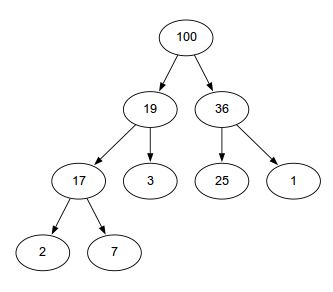
\includegraphics[height=120px,width=120px]{poglavlja/slike/heap.png}
\caption{Zadatak \ref{4_26}}
\label{fig:zadatak426}
\endminipage\hfill
\minipage{0.425\textwidth}
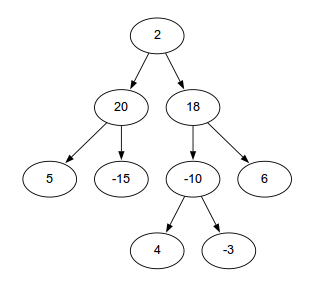
\includegraphics[height=120px,width=120px]{poglavlja/slike/binarna_stabla.png}
\caption{Zadatak \ref{4_27}}
\label{fig:zadatak427}
\endminipage\hfill

\end{figure}

%11.zadatak
%nije resen
\skrati{2}
\begin{Exercise}[label=4_27]
Dato je binarno stablo celih brojeva.
\skrati{1}
\begin{enumerate}
\item Napisati funkciju koja pronalazi čvor u stablu sa najvećim zbirom vrednosti iz desnog podstabla.
\skrati{1}
\item Napisati funkciju koja pronalazi čvor u stablu sa najmanjim zbirom vrednosti iz levog podstabla.
\skrati{1}
\item Napisati funkciju koja štampa sadržaj svih čvorova stabla na putanji od korena do najdubljeg čvora.
\skrati{1}
\item Napisati funkciju koja štampa sadržaj svih čvorova stabla na putanji od korena do čvora koji ima najmanju vrednost u stablu.
\end{enumerate}
Napisati program koji testira gore navedene funkcije nad stablom zadatim slikom \ref{fig:zadatak427} i rezultat ispisuje na standardni izlaz.  
%\linkresenje{4_27}

\skrati{2}
\begin{maxitest}
\begin{test}{1}
#\naslovIzlaz#
#\izlaz{Vrednost u cvoru sa maksimalnim desnim zbirom: 18}#
#\izlaz{Vrednost u cvoru sa minimalnim levim zbirom: 18}#
#\izlaz{2 18 -10 4}#
#\izlaz{2 20 -15}#
\end{test}
\end{maxitest}

\end{Exercise}

%\begin{Answer}[ref=4_27]
%\includecode{resenja/4_DinamickeStrukture/4_27.c}
%\end{Answer}

\section{Rešenja}
\shipoutAnswer
